\section{Geometric Reduction}
\showtoc

\subsection{Functional Routhian Reduction}
\frame[t]{ \frametitle{Overview---How to Walk in Five Easy Steps}
  \only<1>{

    \begin{description}[D]

    \item[ Step 1:]  Consider a 2D biped.
    \end{description}


    {\scriptsize
      \begin{diagram}[width=5em,height=5em]
        && \\
        && \\
        \fbox{$\begin{array}{c}$2D Biped$\end{array}$}  &   & \hspace{2cm}\\
      \end{diagram}
    }


  }

  \only<2>{


    \begin{description}[D]

    \item[ Step 2:]  Use an existing controller to obtain stable walking gaits.

    \end{description}

    {\scriptsize
      \begin{diagram}[width=5em,height=5em]
        && \\
        && \\
        \fbox{$\begin{array}{c}$2D Biped$\end{array}$} &
        \rTo^{\mathsf{Sagittal}}_{\mathsf{Control}} &
        \fbox{$\begin{array}{c}$2D Biped$\\$walking stably$\end{array}$} \\
      \end{diagram}
    }



  }

  \only<3>{

    \begin{description}[D]
    \item[ Step 3:]  For a 3D biped, utilize \alert{energy shaping} so that hybrid reduction can be applied.
    \end{description}

    {\scriptsize
      \begin{diagram}[width=5em,height=5em]
        \fbox{$\begin{array}{c}$3D Biped$ \end{array}$} &
        \rTo^{\mathsf{Energy}}_{\mathsf{Shaping}} &
        \fbox{$\begin{array}{c}$3D Biped$\\$amenable to$\\$reduction$\end{array}$} \\
        && \\
        \fbox{$\begin{array}{c}$2D Biped$\end{array}$} &
        \rTo^{\mathsf{Sagittal}}_{\mathsf{Control}} &
        \fbox{$\begin{array}{c}$2D Biped$\\$walking stably$\end{array}$} \\
      \end{diagram}
    }



  }

  \only<4>{

    \begin{description}[D]
    \item[ Step 4:]  Apply \alert{hybrid reduction}---the reduced system is the 2D biped
      with walking gaits.
    \end{description}


    {\scriptsize
      \begin{diagram}[width=5em,height=5em]
        \fbox{$\begin{array}{c}$3D Biped$ \end{array}$} &
        \rTo^{\mathsf{Energy}}_{\mathsf{Shaping}} &
        \fbox{$\begin{array}{c}$3D Biped$\\$amenable to$\\$reduction$\end{array}$}\\ &&
        \uTo  \dTo_{\begin{array}{c}$Hybrid$\\$Reduction$\end{array}} \\
        \fbox{$\begin{array}{c}$2D Biped$\end{array}$} &
        \rTo^{\mathsf{Sagittal}}_{\mathsf{Control}}  &  \fbox{$\begin{array}{c}$2D Biped$\\$walking stably$\end{array}$}\\
      \end{diagram}
    }


  }

  \only<5>{

    \begin{description}[D]
    \item[ Step 5:]  Utilize \alert{feedback linearization} and \alert{hybrid zero dynamics} to stabilize
      the unstable walking gaits.
    \end{description}


    {\scriptsize
      \begin{diagram}[width=5em,height=5em]
        \fbox{$\begin{array}{c}$3D Biped$ \end{array}$} &
        \rTo^{\mathsf{Energy}}_{\mathsf{Shaping}} &
        \fbox{$\begin{array}{c}$3D Biped$\\$amenable to$\\$reduction$\end{array}$} &
        \rTo^{\mathsf{Hybrid}}_{\mathsf{Zero \:\:  Dynamics}} &
        \fbox{$\begin{array}{c}$3D Biped$\\$walking stably$\end{array}$}\\ &&
        \uTo \dTo_{\begin{array}{c}$Hybrid$\\$Reduction$\end{array}} && \\
        \fbox{$\begin{array}{c}$2D Biped$\end{array}$} &
        \rTo^{\mathsf{Sagittal}}_{\mathsf{Control}} &
        \fbox{$\begin{array}{c}$2D Biped$\\$walking stably$\end{array}$} && \\
      \end{diagram}
    }



  }

  \only<6>{
    \begin{block}{The End Result}
      A control law that that yields stable walking gaits for a 3D biped, given stable walking gaits for a planar equivalent 2D biped.
    \end{block}
           {\scriptsize
             \begin{diagram}[width=5em,height=5em]
               \fbox{$\begin{array}{c}$3D Biped$ \end{array}$} &
               \rTo^{\mathsf{Energy}}_{\mathsf{Shaping}} &
               \fbox{$\begin{array}{c}$3D Biped$\\$amenable to$\\$reduction$\end{array}$} &
               \rTo^{\mathsf{Hybrid}}_{\mathsf{Zero \:\:  Dynamics}} &
               \fbox{$\begin{array}{c}$3D Biped$\\$walking stably$\end{array}$}\\ &&
               \uTo \dTo_{\begin{array}{c}$Hybrid$\\$Reduction$\end{array}} && \\
               \fbox{$\begin{array}{c}$2D Biped$\end{array}$} &
               \rTo^{\mathsf{Sagittal}}_{\mathsf{Control}} &
               \fbox{$\begin{array}{c}$2D Biped$\\$walking stably$\end{array}$} && \\
             \end{diagram}
           }
  }

}

\begin{frame}
  \frametitle{Setup}
  \begin{description}[D]
  \item[ Geometric reduction\footnote{For more on geometric reduction, see [Marsden, Springer-Verlag 1994]}:] \hspace{5cm}

    \begin{itemize}
    \item Begin with a Lagrangian $\Lagrangian : T\ConfigurationSpace \to \R$.
    \item Symmetries in the system are characterized by \textcolor{blue}{cyclic}
      variables: $\frac{\partial \Lagrangian}{\partial \phi} = 0$.
    \item The dimensionality of the phase space can be reduced (by ``dividing'' out by the symmetries).
    \item A corresponding Lagrangian, the \textcolor{blue}{Routhian}, can be defined on this reduced phase space.
    \end{itemize}
  \end{description}

  \begin{block}{Geometric Reduction ``Theorem''}
    One can understand the behavior of the full-order system in terms of
    the behavior of the reduced system and vice versa.
  \end{block}
\end{frame}

\begin{frame}
  \frametitle{Motivation}
  \begin{description}[D]
  \item[ Classical Reduction:]  The conserved quantities used to reduce and reconstruct systems are constants.
  \item[ Yet:]  It may be desirable to \alert{vary} the cyclic variables while not affecting the reduced order system.
  \item[ Motivates:]  An extension of Routhian reduction, termed \alert{functional Routhian reduction}, where the conserved quantities are functions of the cyclic variables:
    \begin{itemize}
    \item Allows us to control the cyclic variables.
    \item Can be effectively used to reduce bipedal robotic walkers.
    \item Generalizes to hybrid systems.
    \end{itemize}
  \end{description}
\end{frame}

\begin{frame}
  \frametitle{Almost-Cyclic Lagrangians \& Functional Routhians}
  \vspace{-1mm}

  Consider the case when $\ConfigurationSpace = S \times \S$ where $S$ is called the \textcolor{blue}{shape space}; we denote an element $q \in \ConfigurationSpace$ by $q = (\theta^T, \varphi)^T$.

  \vspace{-1mm}

  \begin{definition}
    A Lagrangian $\Llambda : TS \times T\S \to \R$ is \alert{almost-cyclic} if:
    \vspace{-3mm}
    \begin{align*}
      \Llambda(\theta, \phi, \dot \theta, \dot \phi)  =
      \frac{1}{2} \left(\!\!\begin{array}{cc}
      \dot \theta^T  &  \dot \phi
      \end{array}\!\!\right) \Mlambda(\theta)
      \left(\begin{array}{c}
        \dot \theta\\
        \dot \phi
      \end{array}\right) - \Wlambda(\theta, \phi, \dot \theta) - \Vlambda(\theta, \phi),
    \end{align*}
    for some function $\lambda : \S \to \R$.
  \end{definition}

  \only<1>{
    \vspace{-7mm}
    \textcolor{darkgray}{
      \begin{align*}
        \Mlambda(\theta) &= \left(\begin{array}{cc}
          \textcolor{lightblue}{\Mtheta(\theta)} + \Mphitheta^T(\theta) \Mphi^{-1}(\theta) \Mphitheta(\theta) & \Mphitheta^T(\theta)\\
          \Mphitheta(\theta) \qquad & \Mphi(\theta)
        \end{array}\right),\\[0mm]
        \Wlambda(\theta,\phi,\dot \theta) &= \textcolor{berkeleygold}{\lambda(\varphi)} \Mphi^{-1}(\theta) \Mphitheta(\theta) \dot{\theta},\\[0mm]
        \Vlambda(\theta,\phi) &= \textcolor{lightblue}{\Vt(\theta)} - \frac{1}{2} \textcolor{berkeleygold}{\lambda(\varphi)} \Mphi^{-1}(\theta) \textcolor{berkeleygold}{\lambda(\varphi)}.
      \end{align*}
    }
  }

  \only<2>{
    \begin{definition}
      The corresponding \alert{ functional Routhian} $\Lt : TS \to \R$ is: \vspace{-.3cm}
      \begin{eqnarray*}
        \Lt(\theta, \dot \theta) &=& \left[ \Llambda(\theta, \varphi, \dot{\theta}, \dot{\varphi}) - \lambda(\varphi) \dot{\varphi} \right]_{\Jfcn = \lambda(\varphi)}\\[0mm]
        & = &  \frac{1}{2} \dot{\theta}^T M_\theta(\theta) \dot{\theta} - \Vt(\theta).
      \end{eqnarray*}
    \end{definition}
  }
\end{frame}

\begin{frame}
  \frametitle{Functional Routhian Reduction}

  \begin{theorem}
    {\small Let $\Llambda$ be an almost-cyclic Lagrangian with an almost-cyclic variable, $\varphi$, and $\Lt$ the corresponding functional Routhian with shape space $S = \R^{n - 1}$. Let $\Upsilon : TS \times \S \to \R^n$ represent external forces satisfying:
      \begin{enumerate}
      \item $\Fextt$ does not depend on $\varphi,\dot{\varphi}$,
      \item $\Upsilon_i(\theta,\dot{\theta}) = 0$ for $i = 2, \ldots, n$.
      \end{enumerate}
      Then $(\theta(t), \varphi(t), \dot{\theta}(t), \dot{\varphi}(t))$ is a solution to the forced vector field $f_{\Llambda}$ on $[t_0, t_F]$ with \vspace{-2mm}
      \begin{align*}
        \dot{\varphi}(t_0) = \Mphi^{-1}(\theta(t_0)) (\lambda(\varphi(t_0)) - \Mphitheta(\theta(t_0))\dot{\theta}(t_0)),\\[-7mm]
      \end{align*}
      if and only if $(\theta(t), \dot{\theta}(t))$ is a solution to the forced vector field $f_{\Lt}$ and $(\varphi(t), \dot{\varphi}(t))$ satisfies:\vspace{-2mm}
      \begin{align*}
        \dot{\varphi}(t) = \Mphi^{-1}(\theta(t)) (\lambda(\varphi(t)) - \Mphitheta(\theta(t))\dot{\theta}(t)).\\[-1.2cm]
    \end{align*}}
  \end{theorem}
\end{frame}



%%%%
\subsection{Reduction Control Laws}
\frame[t] {
  \frametitle{Sagittal Control Law: Reduced Dynamics Controller}

  Consider the sagittal restriction of the 3D biped, which will be a 2D biped, and apply a 2D controller that results in stable walking for this system.

  \only<1> {
    \begin{columns}
      \begin{column}{0.3\textwidth}
        \begin{figure}
          \centering
          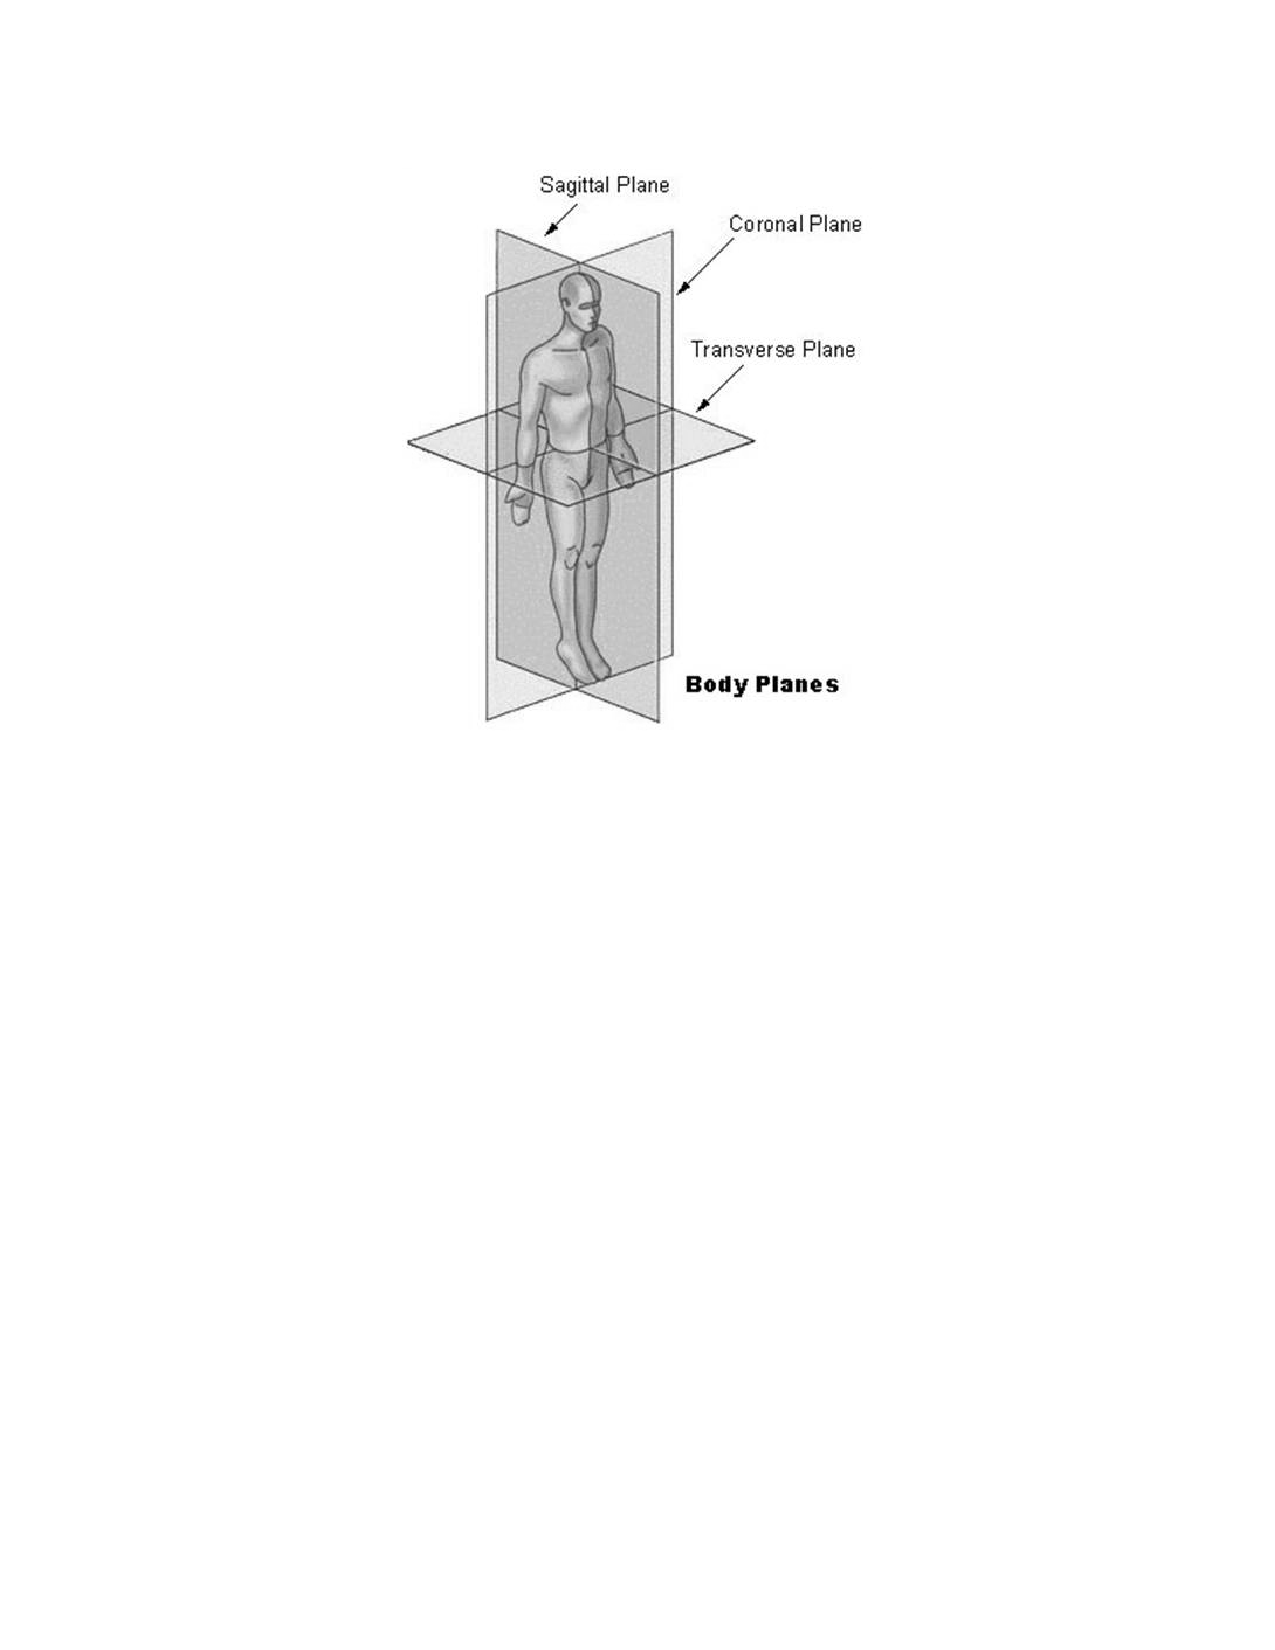
\includegraphics[height=4cm]{bodyplanes}
        \end{figure}
      \end{column}
      \begin{column}{0.6\textwidth}
        \begin{figure}
          \centering
          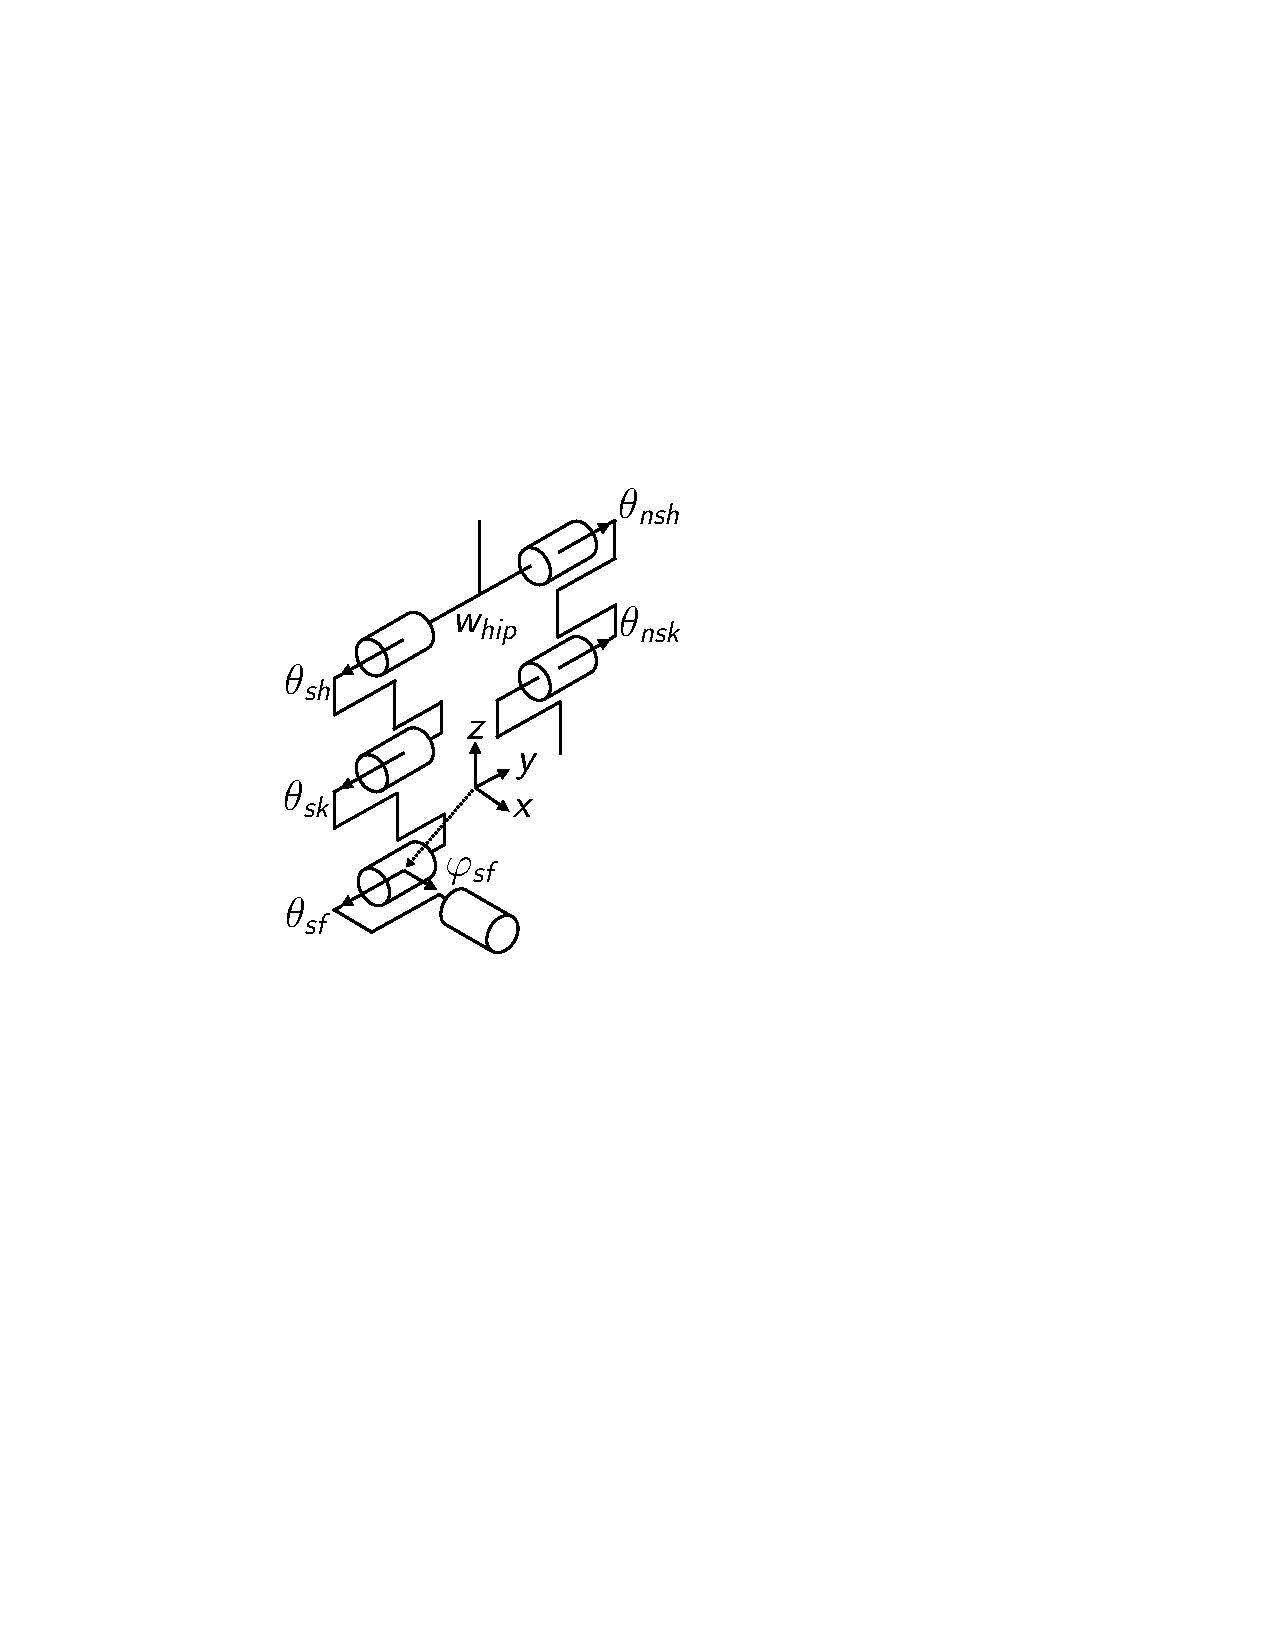
\includegraphics[height=3cm]{robot_angles_3d} \qquad
          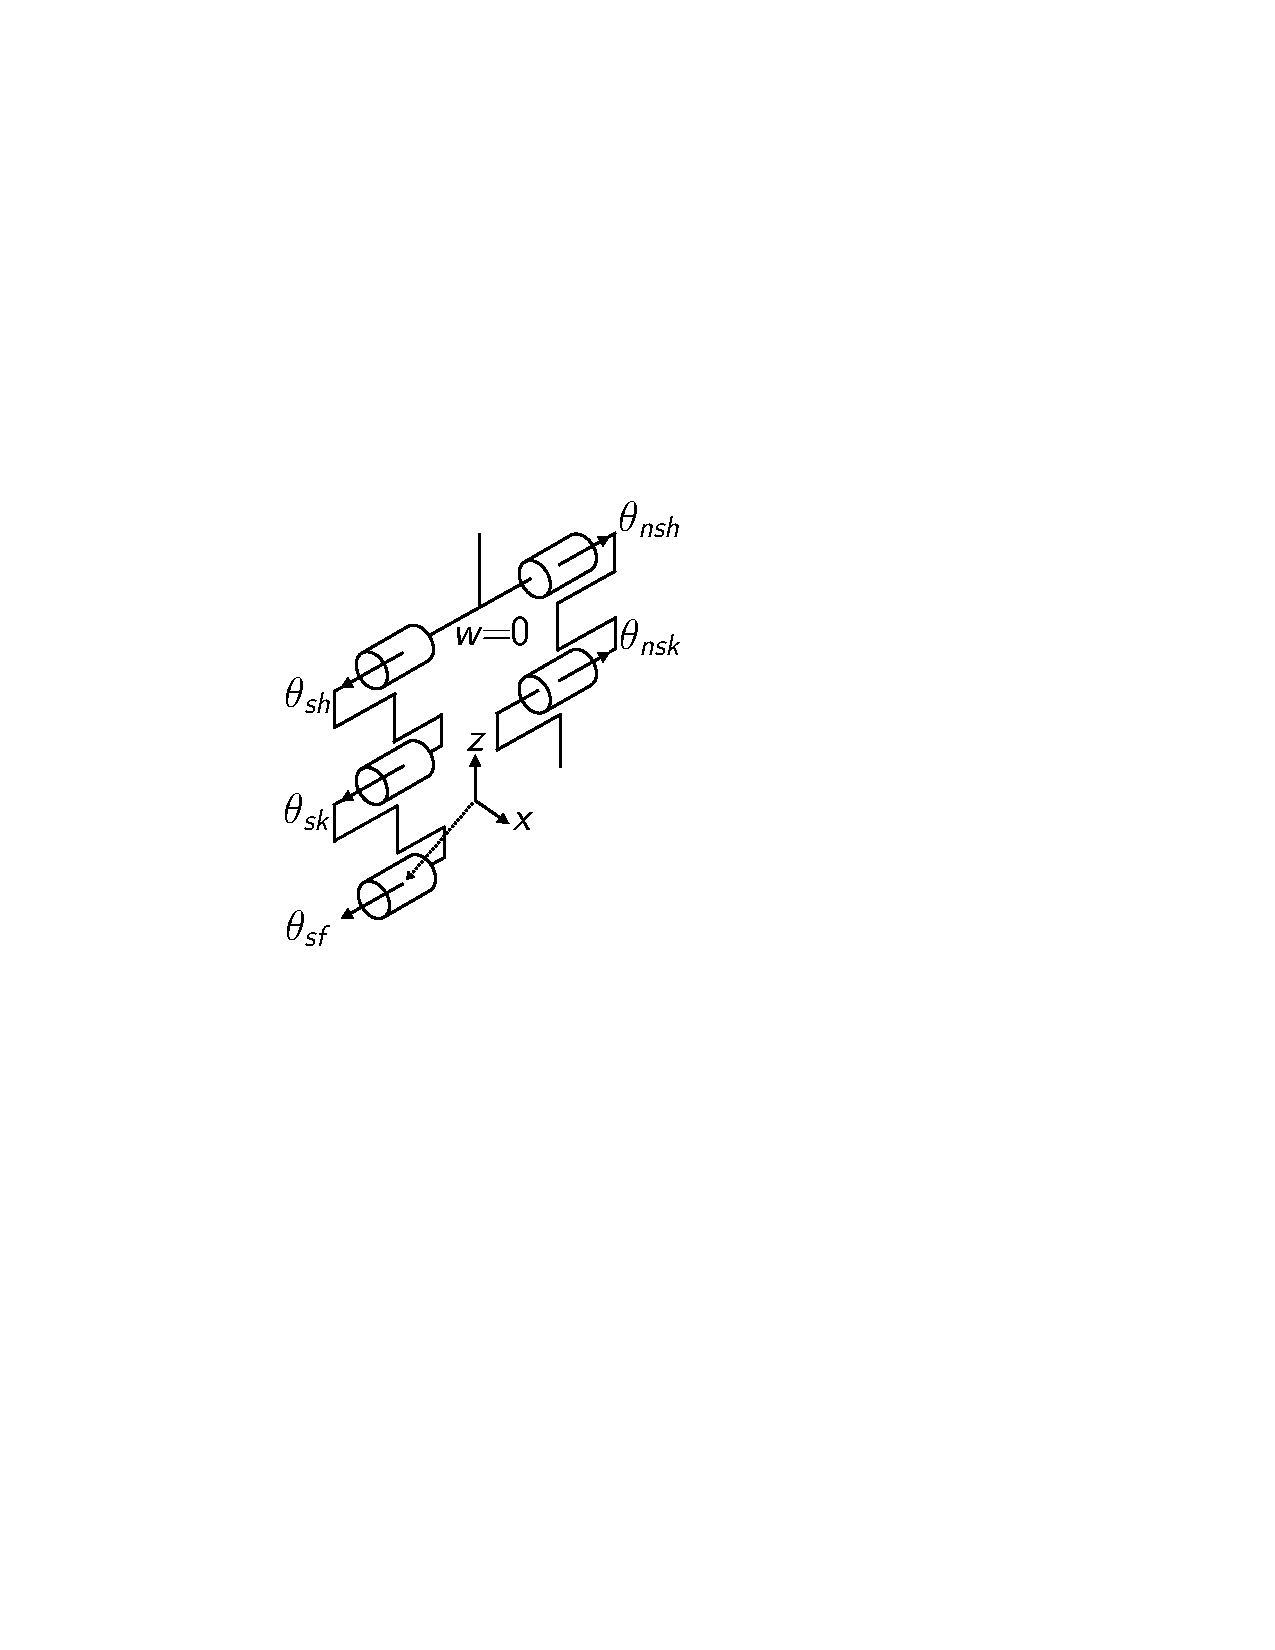
\includegraphics[height=3cm]{robot_angles_2d}
          \caption{Sagittal restriction of of 3D biped leads to a reduced model.}
        \end{figure}
      \end{column}
    \end{columns}
  }

  \only<2> {
    {\scriptsize  \textcolor{gray}{
        \begin{diagram}[width=5em,height=5em]
          \textcolor{black}{\fbox{$\begin{array}{c}$Hipped 3D Biped$\end{array}$}} &
          \rTo^{1^{\mathsf{st}} \:\: \mathsf{Reduction}}_{\mathsf{Control} \:\: \mathsf{Law}} &
          \fbox{$\begin{array}{c}$3D Biped$\\$with shaped$\\$energy$\end{array}$} &
          \rTo^{2^{\mathsf{nd}} \:\: \mathsf{Reduction}}_{\mathsf{Control} \:\: \mathsf{Law}} &
          \fbox{$\begin{array}{c}$3D Biped$\\$walking stably$\end{array}$}\\
          \dDashto^{\textcolor{black}{\mathsf{Sagittal}}}_{\textcolor{black}{\mathsf{Restriction}}} &&
          \uTo \dTo_{\begin{array}{c}$Reduction$\end{array}}&&\\
          \textcolor{black}{\fbox{$\begin{array}{c}$2D Biped$\end{array}$}} &
          \rTo^{\textcolor{black}{\mathsf{Sagittal}}}_{\textcolor{black}{\mathsf{Control} \:\: \mathsf{Law}}} &
          \textcolor{black}{\fbox{$\begin{array}{c}$2D Biped$\\$walking stably$\end{array}$}} && \\
    \end{diagram}}}
  }

  \only<3> {
    \begin{itemize}
    \item  The Lagrangian of the 3D biped has the general form:
      \begin{eqnarray}
        \label{eq:submats}
        \lefteqn{\Lfd(\cq{},\cdq{}) = -\Vu \ + }\\
        \nonumber
        &&\frac{1}{2}
        \left(\begin{array}{c c}
          \dot{\theta}^T & \dot{\varphi}
        \end{array}\right)
        \underbrace{\left(\begin{array}{c c}
            \Mth & \Mphitheta^T(\theta,\varphi)\\
            \Mphitheta(\theta,\varphi) & \Mphi(\theta,\varphi)
          \end{array}\right)}_{\mMu}
        \left(\begin{array}{c}
          \dot{\theta}\\
          \dot{\varphi}
        \end{array}\right), \nonumber
      \end{eqnarray}
      \vspace{-5mm}

    \item The Lagrangian of the sagittal restriction is given by:
      \begin{align*}
        \Lrd(\theta,\dot{\theta}) = \frac{1}{2} \dot{\theta}^T \Mth \dot{\theta} - \left.\Vu\right\vert_{\varphi=0},
      \end{align*}

    \end{itemize}
  }

  \only<4> {
    \vspace{-.1cm}
    \begin{itemize}

    \item The Lagrangian of the sagittal restriction is given by:
      \begin{align*}
        \Lrd(\theta,\dot{\theta}) = \frac{1}{2} \dot{\theta}^T \Mth \dot{\theta} - \left.\Vu\right\vert_{\varphi=0},
      \end{align*}

    \item This yields a control system: $(\fr,\gr)$.

    \item \alert{Assume} there exists a control law, $\usagarg$, that results in stable 2D waking for the dynamical system:
      \begin{align*}
        \flt = \fr(\theta, \dot{\theta}) + \gr(\theta) \usagarg.
      \end{align*}

    \end{itemize}
  }

  %\only<5> {
  %  \begin{figure}
  %    \centering
  %    \movie[width=0.6\textwidth,externalviewer]{
  %    \includegraphics[width=0.6\textwidth]{2dwalkinggait.pdf}}{Movies/2d-movie.avi}\\
  %    \includegraphics[height=0.3\textheight]{pp-2d-legs.pdf}
  %    \includegraphics[height=0.3\textheight]{pp-2d-feet.pdf}
  %  \end{figure}
  %}
  %
}

\frame[t] {
  \frametitle{$1^{\mathsf{st}}$ Reduction Control Law: Lagrangian Shaping Controller}

  Shape the total energy of the 3D biped so that functional Routhian reduction can be applied and the reduced system is exactly the 2D system obtained from the first control law.

  {\scriptsize \textcolor{gray}{
      \begin{diagram}[width=5em,height=5em]
        \textcolor{black}{\fbox{$\begin{array}{c}$Hipped 3D Biped$ \end{array}$}} &
        \rTo^{\textcolor{black}{1^{\mathsf{st}} \:\: \mathsf{Reduction}}}_{\textcolor{black}{\mathsf{Control} \:\: \mathsf{Law}}} &
        \textcolor{black}{\fbox{$\begin{array}{c}$3D Biped$\\$with shaped$\\$energy$\end{array}$}} &
        \rTo^{2^{\mathsf{nd}} \:\: \mathsf{Reduction}}_{\mathsf{Control} \:\: \mathsf{Law}} &
        \fbox{$\begin{array}{c}$3D Biped$\\$walking stably$\end{array}$}\\
        \dDashto^{\textcolor{black}{\mathsf{Sagittal}}}_{\textcolor{black}{\mathsf{Restriction}}} &&
        \uTo \dTo_{\textcolor{black}{\begin{array}{c}$Reduction$\end{array}}}&&\\
        \textcolor{black}{\fbox{$\begin{array}{c}$2D Biped$\end{array}$}} &
        \rTo^{\textcolor{black}{\mathsf{Sagittal}}}_{\textcolor{black}{\mathsf{Control} \:\: \mathsf{Law}}} &
        \textcolor{black}{\fbox{$\begin{array}{c}$2D Biped$\\$walking stably$\end{array}$}} &&
      \end{diagram}
  }}
}


\frame[t] {
  \frametitle{$2^{\mathsf{nd}}$ Reduction Control Law: Zero Dynamics Controller}

  Use feedback linearization to stabilize to the surface of initial conditions for which the decoupling promised by functional Routhian Reduction is valid.

  {\scriptsize  \textcolor{gray}{
      \begin{diagram}[width=5em,height=5em]
        \textcolor{black}{\fbox{$\begin{array}{c}$Hipped 3D Biped$\end{array}$}} &
        \rTo^{\textcolor{black}{1^{\mathsf{st}} \:\: \mathsf{Reduction}}}_{\textcolor{black}{\mathsf{Control} \:\: \mathsf{Law}}} &
        \textcolor{black}{\fbox{$\begin{array}{c}$3D Biped$\\$with shaped$\\$energy$\end{array}$}} &
        \rTo^{\textcolor{black}{2^{\mathsf{nd}} \:\: \mathsf{Reduction}}}_{\textcolor{black}{\mathsf{Control} \:\: \mathsf{Law}}} &
        \textcolor{black}{\fbox{$\begin{array}{c}$3D Biped$\\$walking stably$\end{array}$}}\\
        \dDashto^{\textcolor{black}{\mathsf{Sagittal}}}_{\textcolor{black}{\mathsf{Restriction}}} &&
        \uTo \dTo_{\textcolor{black}{\begin{array}{c}$Reduction$\end{array}}}&& \\
        \textcolor{black}{\fbox{$\begin{array}{c}$2D Biped$\end{array}$}} &
        \rTo^{\textcolor{black}{\mathsf{Sagittal}}}_{\textcolor{black}{\mathsf{Control} \:\: \mathsf{Law}}} &
        \textcolor{black}{\fbox{$\begin{array}{c}$2D Biped$\\$walking stably$\end{array}$}}&&
      \end{diagram}
  }}
}

\begin{frame}
  \frametitle{Combining ES and FRR}
  \only<1>{
    \begin{columns}
      \column{1.5in}
      Dynamic Model:
      \begin{align*}
        M(q) \ddot q + H(q, \dot q) = 0
      \end{align*}
      Control Law:
      \begin{align*}
        u &= G(q) - G(\Psi(q),\\
        u_2 &=-k_{d} (\dot \vartheta_{T}^{a})\\
        &\hspace{1.8em} -k_{p} (\vartheta_{T}^{a} - \vartheta_{T}^{d}).
      \end{align*}
      \column{1.5in}
      \begin{figure}
        \centering
        \def\svgwidth{1.0\columnwidth}
        \input{figures/cg2d-3link-model.eps_latex}
        \vspace{-2em}
        \caption{3D 3-link biped configuration, $\varphi$ ommited for clarity).}
      \end{figure}
    \end{columns}
  }
  \only<2>{
    \begin{figure}
      \centering
      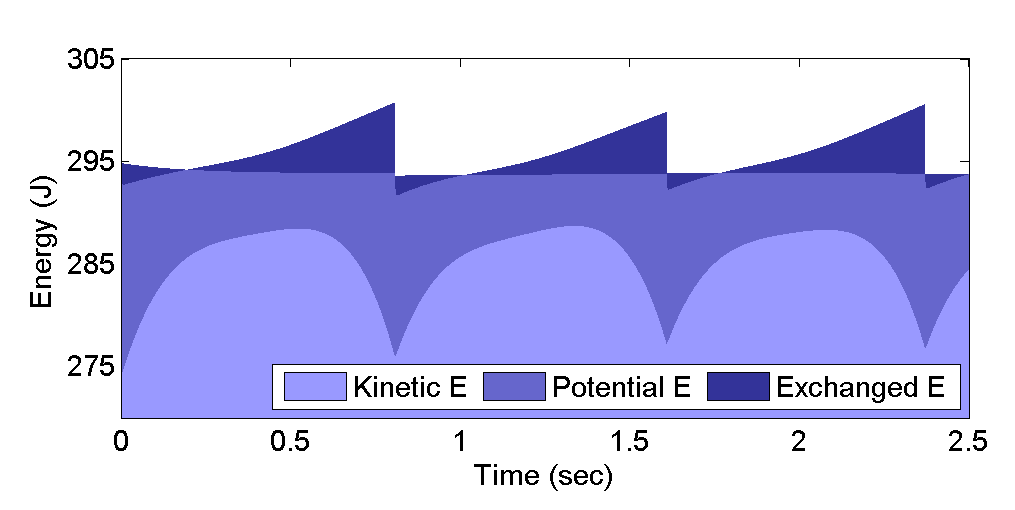
\includegraphics[width=1.0\columnwidth]{energy_conserved_cg3d_3link}
      \caption{The quantity, $E_{0} \equiv T(q, \dot q) + V(q) + \int_{t_0}^{t} F_{nc} \cdot \frac{d\q}{d\tau} d\tau$, is conserved.}
    \end{figure}
  }
  \only<3>{
    \begin{figure}
      \centering
      \includemedia[
        %width=1.0\columnwidth,
        %height=0.5625\columnwidth,
        width=1.0\columnwidth,
        height=0.5\columnwidth,
        addresource=3d_3link_es_frr.mp4,
        activate=pageopen,
        flashvars={source=3d_3link_es_frr.mp4&loop=true&autoPlay=true}
      ]{}{VPlayer9.swf}
      \caption{Converging to the gait with energy shaping.}
    \end{figure}
  }
\end{frame}
